\chapter{Test af UDP-server og client}\label{ch:test}
UDP-clienten og serveren blev testet ved at sende diverse kommandoer fra serveren på den ene virtuelle maskine til clienten den anden virtuelle maskine.

\noindent Nedenfor ses nogle eksempler på overførelser:

		\begin{figure}[H]
			\centering
			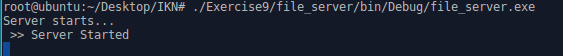
\includegraphics[width=160mm]{figures/Serverstartup.png}
			\caption{Serveren når den startes}
		\end{figure}

		\begin{figure}[H]
			\centering
			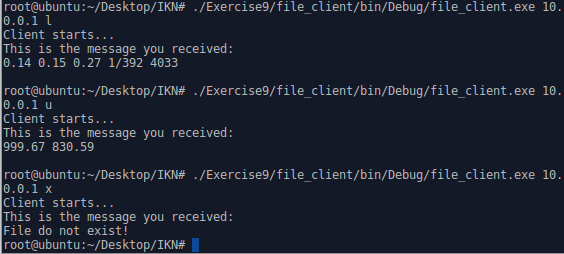
\includegraphics[width=160mm]{figures/clientrequests.png}
			\caption{Eksempler på kommandoer sendt fra clienten}
		\end{figure}

\noindent Som det kan ses på ovenstående figurer kører serveren iterativt. Efter serveren er blevet startet bliver den ved med at køre og lytte efter clients. Clients kan så kalde applikationen med parameterene <ip-adresse> <kommando>, hvorefter serveren læser henholdsvis "/proc/loadavg" eller "/proc/uptime" og sender indholdet til clienten. Ellers reutneres en fejlbesked. Efter filen er blevet modtaget lukker clienten forbindelsen, og en ny client kan komme til.